\documentclass[10.5pt,a4paper]{article}
\usepackage[T1]{fontenc}
\usepackage{charter}
\usepackage[scaled=0.92]{helvet}
\usepackage[a4paper,top=20mm,bottom=18mm,left=21mm,right=21mm,headsep=8mm]{geometry}
\usepackage{microtype}
\usepackage{enumitem,titlesec,tabularx,booktabs,array,graphicx,lastpage,fancyhdr}
\usepackage[table]{xcolor}
\usepackage[hidelinks]{hyperref}
\usepackage{caption}

\definecolor{accent}{HTML}{1F3F7A}
\definecolor{mute}{HTML}{6B7180}
\setlength{\parindent}{0pt}
\setlength{\parskip}{5pt}
\linespread{1.08}

\pagestyle{fancy}\fancyhf{}
\renewcommand{\headrulewidth}{0.4pt}
\fancyhead[L]{\footnotesize\sffamily\color{mute}DongGeon (Lloyd) Kwak}
\fancyhead[R]{\footnotesize\sffamily\color{mute}Career Description}
\fancyfoot[R]{\footnotesize\sffamily\color{mute}\thepage\ / \pageref{LastPage}}

\titleformat{\section}{\sffamily\bfseries\Large\color{accent}}{}{0pt}{}
\titlespacing*{\section}{0pt}{4pt}{4pt}
\titleformat{\subsection}{\sffamily\bfseries\footnotesize\color{accent}}{}{0pt}{\MakeUppercase}
\titlespacing*{\subsection}{0pt}{10pt}{2pt}
\setlist[itemize]{leftmargin=13pt,topsep=1pt,itemsep=3pt,parsep=0pt,label={\small\textbullet}}
\captionsetup{font={small,it},labelformat=empty,skip=4pt}

% one line of facts under each title
\newcommand{\facts}[1]{{\small\color{mute}#1}\par\vspace{2pt}}

\begin{document}

% ---------------------------------------------------------------- PROFILE
\begin{minipage}[t]{0.76\linewidth}\vspace{0pt}
  {\sffamily\bfseries\fontsize{24}{28}\selectfont DongGeon (Lloyd) Kwak}\\[6pt]
  {\large B.E.\ Computer Science and Engineering, SeoulTech}\\[3pt]
  {\small\color{mute}kwaklloyd@gmail.com \;\textbullet\; lloydkwak.github.io \;\textbullet\; github.com/lloydkwak}
\end{minipage}\hfill
\begin{minipage}[t]{0.17\linewidth}\vspace{0pt}\raggedleft
  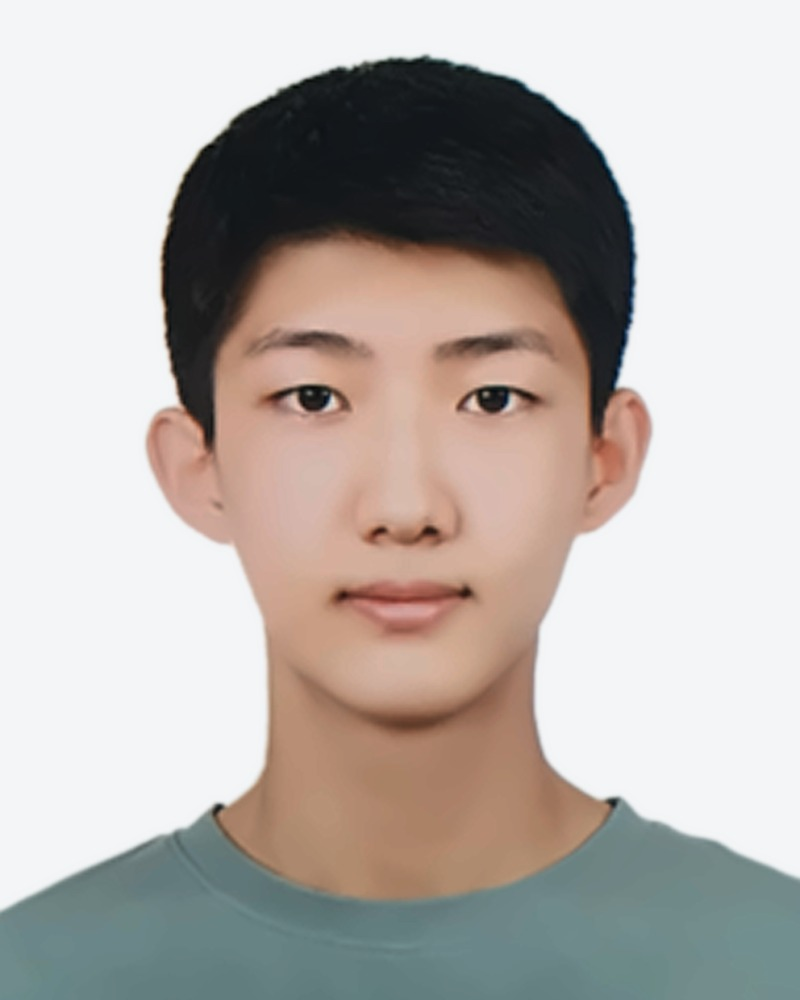
\includegraphics[width=\linewidth]{profile.jpg}
\end{minipage}

\subsection{Profile}
Fourth-year undergraduate in Computer Science and Engineering (minor in Applied AI), graduating in August 2027; GPA 4.13/4.50, 8th of 114 in major. I study how pretrained robot policies can keep working when the robot's body changes. Before that I worked as a software developer at two companies for eight months.

\subsection{Research interests}
Generalist robot learning \textbullet\ cross-embodiment learning \textbullet\ lifelong robot learning (adaptation, failure detection and recovery) \textbullet\ long-horizon manipulation with task and motion planning

\subsection{Overview}
\renewcommand{\arraystretch}{1.4}
\small
\begin{tabularx}{\linewidth}{@{}p{0.15\linewidth}>{\raggedright}p{0.30\linewidth}>{\raggedright\arraybackslash}X@{}}
\toprule
\textbf{Period} & \textbf{Work} & \textbf{Context}\\
\midrule
2025 -- now & FAVOR & Robot learning research; first-author manuscript in preparation\\
2026 -- now & MTREA & Capstone Design project, two-person team\\
2026 & MakeYourBrick & SeoulTech ST startup club\\
2025 & RL-Arena & Open Source Software course, two-person team; outstanding project\\
2025 & AI-generated image detection & Team project, two people\\
2025 & Logisim MLP & Digital Logic and Systems course; outstanding project\\
2022 -- 2023 & Laver, CHASER & Software developer\\
\bottomrule
\end{tabularx}
\normalsize\renewcommand{\arraystretch}{1}

\subsection{Publications and patents}
\begin{itemize}
  \item \textbf{D.\ Kwak}. FAVOR: Fault-Aware Visuomotor Policy Adaptation via Ordered Retargeting. Manuscript in preparation.
  \item K.\ Lee, G.\ Lee, \textbf{D.\ Kwak}. Real-time crack detection system for construction sites. Korean Patent 10-2647135, registered March 2024.
\end{itemize}

\newpage
% ---------------------------------------------------------------- FAVOR
\section{FAVOR}
\facts{Jul.\ 2025 -- present \textbullet\ Research feedback: Prof.\ Ji-Hyeong Han; weekly lab meetings}

\subsection{Question}
When one joint of a robot arm locks or loses part of its range, can a pretrained diffusion policy still complete its task without retraining, and where should the correction be applied?

\begin{center}
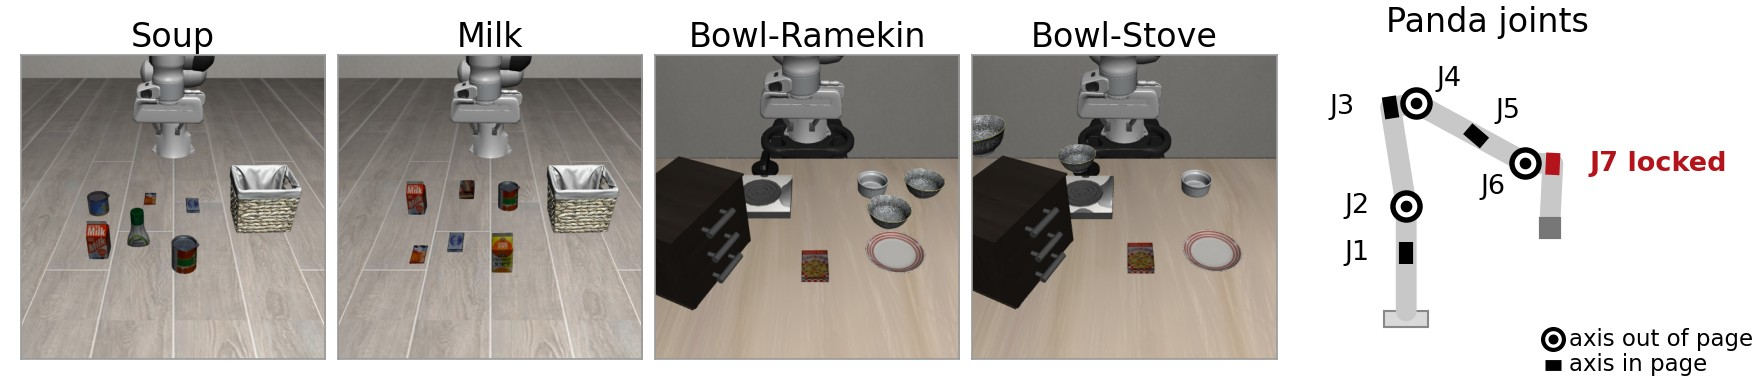
\includegraphics[width=0.94\linewidth]{fig_setup.jpg}
\captionof{figure}{The four simulated tasks (LIBERO) and the Franka Panda joints.}
\end{center}

\subsection{What I did}
\begin{itemize}
  \item Trained a joint-space diffusion policy on a healthy Franka Panda (4 LIBERO tasks) and injected locked and range-limited joint faults at four levels of severity, including faults that appear mid-task.
  \item Compared seven corrections applied at three stages of inference: choosing among sampled actions, guiding the denoising process, and inverse kinematics after sampling. All methods ran on the same seeds and diffusion samples, and the main result was replicated on new seeds.
  \item Found that restoring the end-effector position first, and orientation only with the remaining joints (priority IK), worked best from moderate faults on. Showed that weighted IK without a posture term is equivalent to this to first order, which explains when the weighted baselines fail.
  \item Showed that the end-effector error left after correction predicts which faults are recoverable (AUC 0.94 on the same conditions).
\end{itemize}

\subsection{Results}
\small
\begin{tabularx}{\linewidth}{@{}X*{5}{>{\raggedleft\arraybackslash}p{0.12\linewidth}}@{}}
\toprule
Fault level & No correction & Denoising guidance & Weighted IK (pos.) & Weighted IK (pose) & Priority IK\\
\midrule
Mild & 0.66 & 0.70 & 0.75 & 0.70 & 0.70\\
Moderate & 0.42 & 0.44 & 0.59 & 0.51 & 0.64\\
Severe & 0.28 & 0.31 & 0.45 & 0.39 & 0.58\\
Locked & 0.11 & 0.19 & 0.30 & 0.32 & 0.48\\
\midrule
All 112 conditions & 0.37 & 0.41 & 0.52 & 0.48 & 0.60\\
\bottomrule
\end{tabularx}
\normalsize

{\small\color{mute}Task success rate over 20 paired seeds per condition. Denoising guidance here is the E-C-I projection method.}

\subsection{Limitations}
\begin{itemize}
  \item The method needs an accurate lock angle; a 0.01\,rad error lowers success from 0.67 to 0.39, so the angle should come from the joint encoder.
  \item Some faults (locked joints 2 and 4) cannot be compensated by any of the methods.
  \item All results so far are in simulation. I am now testing on a real xArm7.
\end{itemize}

\newpage
\begin{center}
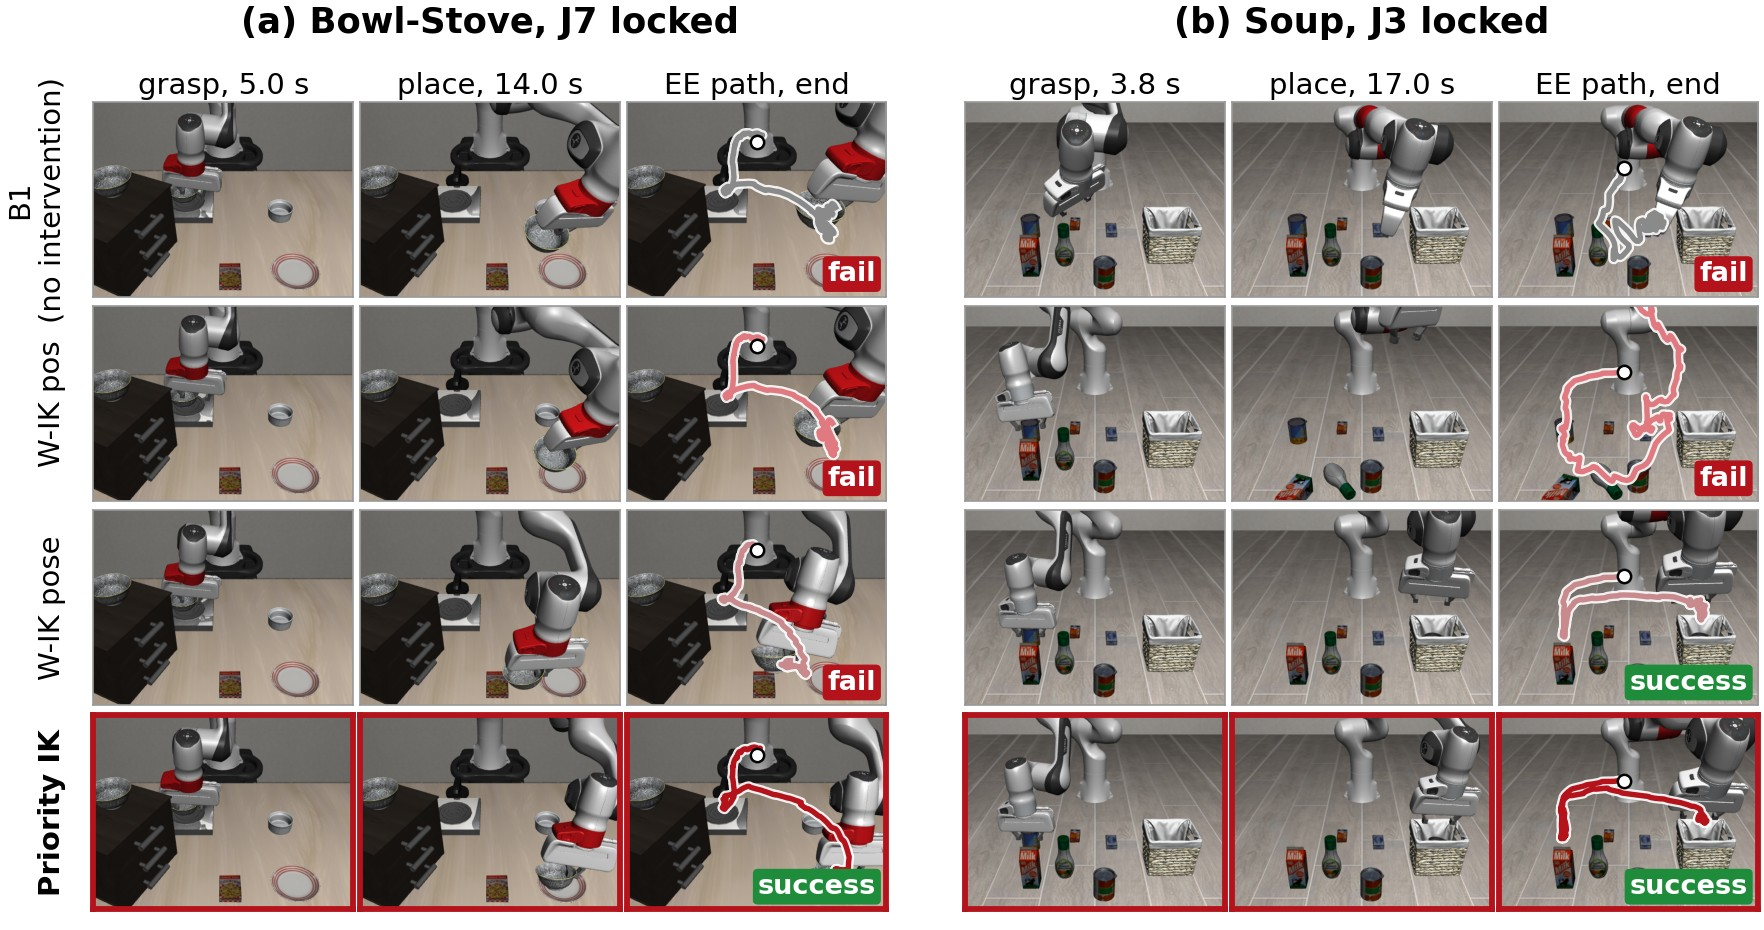
\includegraphics[width=\linewidth]{fig_qual.jpg}
\captionof{figure}{FAVOR: the same episode under four methods for two faults. The bottom row (Priority IK) succeeds in both.}
\end{center}

\vspace{6pt}
% ---------------------------------------------------------------- MTREA
\section{MTREA}
\facts{Sep.\ 2026 -- present \textbullet\ Capstone Design, SeoulTech \textbullet\ two-person team}

\subsection{Question}
When the $\pi_{0.5}$ model is fine-tuned on one task with a new low-cost robot arm (SO-101), does it lose performance on other tasks it could do before?

\subsection{What I did}
\begin{itemize}
  \item Wrote the evaluation protocol with my teammate: fine-tune on pick-and-place only, then test on stacking, pushing, pouring and opening a drawer. Zero-shot performance is not a usable baseline because the new body alone keeps it near zero, so naive full fine-tuning is the baseline and a model fine-tuned on each held-out task is the ceiling.
  \item Built arm calibration and leader--follower teleoperation with a safety lock for data collection, a training wrapper with dataset sync and remote job control for the GPU server, and an asynchronous server that runs the trained policy on the arm.
  \item Measured memory use on the shared GPU (an A100 slice with 40\,GB) and chose full fine-tuning with batch size 16, the largest that fits.
\end{itemize}

\subsection{Status}
Data collection, training and deployment work end to end. The evaluation on the held-out tasks is next.

\newpage
% ---------------------------------------------------------------- PROJECTS
\section{Other Projects}

\par\vspace{9pt}{\sffamily\bfseries MakeYourBrick}\quad{\small\color{mute}May 2026, startup club}\par\vspace{2pt}
\begin{minipage}[t]{0.56\linewidth}\vspace{0pt}
A web app that turns a single photo into a LEGO model. The user selects an object, SAM2 segments it, SAM 3D Objects reconstructs it in 3D, and the shape is converted into colored bricks in the LDraw format. Shadows baked into the reconstructed texture produced black bricks, which I fixed by softening shadows before color quantization. The example shown uses 10,263 bricks.
\end{minipage}\hfill
\begin{minipage}[t]{0.40\linewidth}\vspace{0pt}\centering
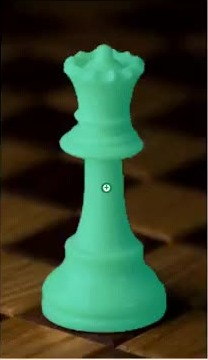
\includegraphics[height=40mm]{myb_demo_crop.jpg}\hspace{2pt}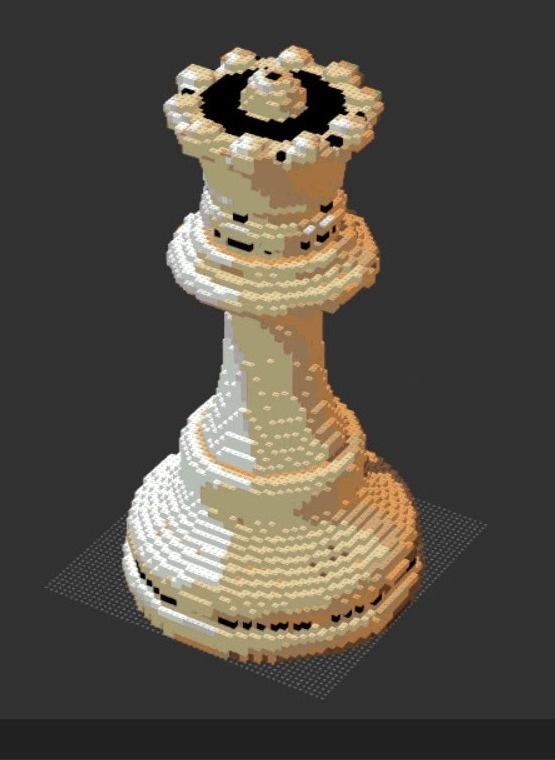
\includegraphics[height=40mm]{myb_ldr_crop.jpg}
\end{minipage}

\par\vspace{9pt}{\sffamily\bfseries RL-Arena}\quad{\small\color{mute}Nov.\ -- Dec.\ 2025, Open Source Software course}\par\vspace{2pt}
A platform where users train reinforcement-learning agents, submit them, and see them ranked by ELO. Two-person team. I built the environment package (published on PyPI as \textit{rl-arena}), the service that runs each match in an isolated container, and most of the backend, including automatic matchmaking; the web interface was shared. Selected as an outstanding project in the course.

\par\vspace{9pt}{\sffamily\bfseries AI-generated image detection}\quad{\small\color{mute}Dec.\ 2025, team of two}\par\vspace{2pt}
A classifier that separates real photos from images made by diffusion models (115k images). Generated images had a narrower spread of pixel intensities, and preprocessing based on this raised test accuracy from 72.6\% to 96.3\% for ResNet-50 and from 60.7\% to 88.9\% for EfficientNet-B4.

\par\vspace{9pt}{\sffamily\bfseries Logisim MLP}\quad{\small\color{mute}Spring 2025, Digital Logic and Systems course}\par\vspace{2pt}
A 256-128-10 MNIST classifier built as a digital logic circuit in Logisim, with about 34,000 trained weights stored in ROM, to understand how a neural network computes at the hardware level. Selected as an outstanding project in the course.

\section{Work Experience}
\facts{Laver, Jun.\ -- Oct.\ 2022 \textbullet\ CHASER, Nov.\ 2022 -- Jan.\ 2023 \textbullet\ software developer}
Developed an object-detection system from model development to product integration, built backend services and APIs, and wrote an IFC-to-XML converter for building information models. I am also a co-inventor (third of three) on a Korean patent for a crack detection system in which mobile robots record video at construction sites and cracks are detected and tracked across frames.

\end{document}
